\documentclass[../main.tex]{subfiles}
\begin{document}

\ifSubfilesClassLoaded{\PageLegaleChapitre}{}

\chapter{Les fonctions et le graphique cartésien}
\label{chap:fonctions-et-graphiques}

% =====================================================
\section{Notion de fonction et repérage cartésien}
% =====================================================

\subsection{Le repère cartésien du plan}
Un repère cartésien du plan est formé de deux axes perpendiculaires qui se croisent en un point appelé l'\textbf{origine} ($0$ ou $O$) :
\begin{itemize}
  \item L'axe horizontal est l'\textbf{axe des abscisses} (généralement l'axe des $x$).
  \item L'axe vertical est l'\textbf{axe des ordonnées} (généralement l'axe des $y$).
\end{itemize}
Chaque point du plan est repéré par un couple de coordonnées $(x; y)$.

\subsection{Qu'est-ce qu'une fonction ?}
\begin{definition}
Une \textbf{fonction} $f$ est un processus qui, à un nombre de départ $x$ (appelé \textbf{antécédent}), associe un \textbf{unique} nombre d'arrivée $y$ (appelé \textbf{image}). On note cela :
\[
f : x \longmapsto f(x) \quad\text{ou}\quad y = f(x)
\]
\end{definition}

% =====================================================
\section{La fonction affine et la fonction linéaire}
% =====================================================

\subsection{La fonction linéaire (proportionnalité)}

\begin{definition}
Une \textbf{fonction linéaire} est de la forme :
\[
f(x) = m \times x \quad (\text{ou } y = mx)
\]
où $m$ est un nombre réel appelé \textbf{coefficient de proportionnalité} (ou pente).
\end{definition}

\textbf{Propriété géométrique :} La représentation graphique d'une fonction linéaire est toujours une \textbf{droite qui passe par l'origine du repère} $(0;0)$.

\subsection{La fonction affine (le cas général)}

\begin{definition}
Une \textbf{fonction affine} est de la forme :
\[
f(x) = mx + p
\]
où :
\begin{itemize}
  \item $m$ est la \textbf{pente} (ou coefficient directeur) de la droite.
  \item $p$ est l'\textbf{ordonnée à l'origine} (l'endroit où la droite coupe l'axe vertical des $y$).
\end{itemize}
\end{definition}

Si $p = 0$, la fonction affine redevient une fonction linéaire ($f(x) = mx$). Si $m = 0$, on obtient une fonction constante ($f(x) = p$, sa représentation est une droite horizontale).

\begin{center}
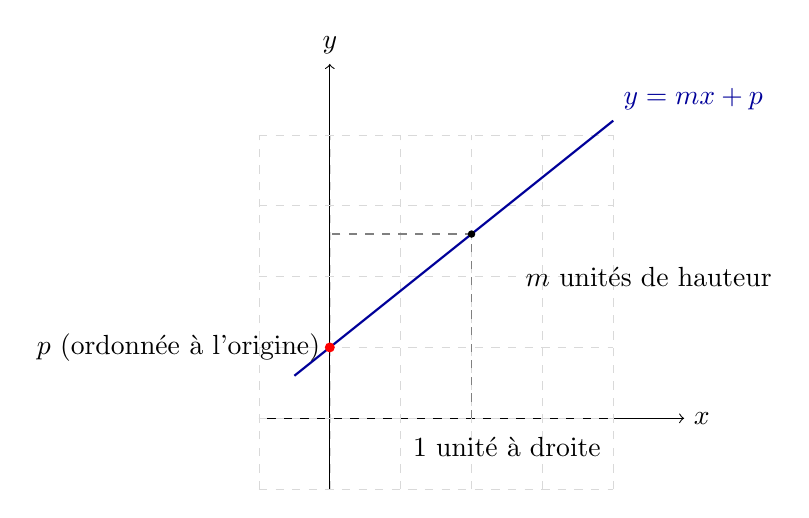
\begin{tikzpicture}[scale=0.9]
  % Axes
  \draw[->] (-1,0) -- (5,0) node[right] {$x$};
  \draw[->] (0,-1) -- (0,5) node[above] {$y$};
  
  % Grille légère
  \draw[help lines, color=gray!30, dashed] (-1,-1) grid (4,4);
  
  % Droite affine y = 0.8x + 1
  \draw[thick, blue!60!black] (-0.5, 0.6) -- (4, 4.2) node[above right] {$y = mx + p$};
  
  % Points et repères
  \fill[red] (0,1) circle (2pt);
  \node[left] at (0,1) {$p$ (ordonnée à l'origine)};
  
  \draw[dashed, gray] (2,0) -- (2,2.6) -- (0,2.6);
  \fill[black] (2,2.6) circle (1.5pt);
  
  \node at (2.5,-0.4) {$1$ unité à droite};
  \node at (4.5,2.0) {$m$ unités de hauteur};
\end{tikzpicture}
\end{center}

% =====================================================
\section{Tracer et déterminer l'équation d'une droite}
% =====================================================

\subsection{Interprétation de la pente $m$}
\begin{propriete}[Rôle de la pente $m$]
La pente $m$ indique comment varie $y$ lorsque $x$ augmente de $1$ unité :
\begin{itemize}
  \item Si \textbf{$m > 0$}, la fonction est \textbf{croissante} (la droite monte vers la droite).
  \item Si \textbf{$m < 0$}, la fonction est \textbf{décroissante} (la droite descend vers la droite).
  \item Plus la valeur absolue de $m$ est grande, plus la droite est « raide ».
\end{itemize}
\end{propriete}

\subsection{Trouver l'équation d'une droite connaissant deux points}

\begin{methode}
Soit une droite passant par deux points $A(x_1; y_1)$ et $B(x_2; y_2)$ :
\begin{enumerate}
  \item Calculer la pente $m$ à l'aide de la formule :
  \[
  m = \frac{y_2 - y_1}{x_2 - x_1}
  \]
  \item Remplacer $m$ dans l'équation $y = mx + p$, puis injecter les coordonnées de l'un des points ($A$ ou $B$) pour résoudre l'équation et trouver $p$.
\end{enumerate}
\end{methode}

\textbf{Exemple :} Trouvons l'équation de la droite passant par $A(1; 3)$ et $B(3; 7)$.
\[
m = \frac{7 - 3}{3 - 1} = \frac{4}{2} = 2.
\]
L'équation est donc de la forme $y = 2x + p$. Utilisons le point $A(1; 3)$ :
\[
3 = 2(1) + p \quad\Longrightarrow\quad 3 = 2 + p \quad\Longrightarrow\quad p = 1.
\]
L'équation de la droite est \textbf{$y = 2x + 1$}.

% =====================================================
\section{Récapitulatif}
% =====================================================

\begin{tcolorbox}[colback=gray!6,colframe=gray!60!black,title={\bfseries À retenir}]
\begin{itemize}
  \item \textbf{Fonction linéaire :} $f(x) = mx$ (passe par l'origine $(0;0)$).
  \item \textbf{Fonction affine :} $f(x) = mx + p$ (représentée par une droite).
  \item \textbf{Pente ($m$) :} $\dfrac{\text{Variation de } y}{\text{Variation de } x} = \dfrac{y_2 - y_1}{x_2 - x_1}$.
  \item \textbf{Ordonnée à l'origine ($p$) :} Valeur de $y$ lorsque $x = 0$ (intersection avec l'axe vertical).
\end{itemize}
\end{tcolorbox}

\newpage
% =====================================================
\section{Exercices}
% =====================================================

\subsection{Série A -- Lecture graphique et calculs d'images}

\begin{enumerate}[label=\textbf{\arabic*.}]

\item Soit la fonction affine définie par $f(x) = -3x + 5$.
\begin{enumerate}[label=\alph*)]
  \item Calcule l'image de $2$ par $f$ (c'est-à-dire $f(2)$).
  \item Calcule l'image de $-1$.
  \item Quel est l'antécédent de $-4$ ? (cherche $x$ tel que $f(x) = -4$).
\end{enumerate}

\item On considère une fonction linéaire $g$ telle que $g(4) = 12$.
\begin{enumerate}[label=\alph*)]
  \item Quel est le coefficient de proportionnalité $m$ de cette fonction ?
  \item Écris l'expression de $g(x)$.
  \item Calcule $g(7)$.
\end{enumerate}

\item Associe chaque fonction à sa description :
\begin{enumerate}[label=\alph*),itemsep=1pt]
  \item $f_1(x) = 2x - 4$ \quad---\quad 1. Décroissante, coupe l'axe des $y$ en $3$.
  \item $f_2(x) = -x + 3$ \quad---\quad 2. Passe par l'origine, croissante.
  \item $f_3(x) = 5x$ \quad\quad\quad\,---\quad 3. Croissante, coupe l'axe des $y$ en $-4$.
\end{enumerate}

\end{enumerate}

\subsection{Série B -- Détermination d'équations de droites}

\begin{enumerate}[label=\textbf{\arabic*.},start=4]

\item Détermine l'équation de la droite $d_1$ qui a une pente $m = 3$ et qui passe par le point $P(2; 5)$.

\item Détermine l'équation de la droite $d_2$ passant par les points $A(2; 1)$ et $B(4; 5)$.

\item Soit une droite d'équation $y = -2x + 6$.
\begin{enumerate}[label=\alph*)]
  \item Cette droite passe-t-elle par le point $C(3; 0)$ ? Justifie par le calcul.
  \item Quelles sont les coordonnées du point d'intersection de cette droite avec l'axe des ordonnées ?
\end{enumerate}

\end{enumerate}

\subsection{Série C -- Problèmes concrets}

\textbf{Mission 1 -- Abonnements téléphoniques.}
L'opérateur A propose un tarif fixe de $20\text{ \euro}$ par mois. L'opérateur B propose un abonnement de base à $10\text{ \euro}$ par mois auquel s'ajoute $0\text{ \euro}\dec 10$ par gigaoctet (Go) consommé.
\begin{enumerate}[label=\alph*)]
  \item Exprime le coût mensuel $C_A(x)$ et $C_B(x)$ en fonction du nombre de Go consommés ($x$).
  \item À partir de combien de Go consommés l'opérateur B devient-il plus cher que l'opérateur A ?
\end{enumerate}

\subsection{Défi bonus}
Trouve l'équation de la droite perpendiculaire à $y = 2x + 1$ (sachant que le produit des pentes de deux droites perpendiculaires vaut $-1$) et qui passe par le point $(4; 5)$.

\newpage
% =====================================================
\section{Corrigés}
% =====================================================

\subsection*{Série A}

\textbf{1.} a) $f(2) = -3(2) + 5 = -6 + 5 = -1$. \quad b) $f(-1) = -3(-1) + 5 = 3 + 5 = 8$. \quad c) $-3x + 5 = -4 \implies -3x = -9 \implies x = 3$.

\textbf{2.} a) $m = \dfrac{12}{4} = 3$. \quad b) $g(x) = 3x$. \quad c) $g(7) = 3 \times 7 = 21$.

\textbf{3.} a $\leftrightarrow$ 3, \quad b $\leftrightarrow$ 1, \quad c $\leftrightarrow$ 2.

\subsection*{Série B}

\textbf{4.} L'équation est $y = 3x + p$. On remplace par $P(2; 5)$ : $5 = 3(2) + p \implies 5 = 6 + p \implies p = -1$. L'équation est $y = 3x - 1$.

\textbf{5.} Pente $m = \dfrac{5 - 1}{4 - 2} = \dfrac{4}{2} = 2$. L'équation est $y = 2x + p$. Avec $A(2; 1)$ : $1 = 2(2) + p \implies 1 = 4 + p \implies p = -3$. L'équation est $y = 2x - 3$.

\textbf{6.} a) On teste $x = 3$ : $y = -2(3) + 6 = -6 + 6 = 0$. Oui, le point $C$ appartient bien à la droite. \quad b) L'ordonnée à l'origine est $6$, donc le point d'intersection est $(0; 6)$.

\subsection*{Série C}

\textbf{Mission 1.} 
a) $C_A(x) = 20$ et $C_B(x) = 0\text{,\!}10x + 10$. \\
b) On cherche quand $C_B(x) > C_A(x)$ : $0\text{,\!}10x + 10 = 20 \implies 0\text{,\!}10x = 10 \implies x = 100$ Go. Dès que l'on dépasse $100$ Go, l'opérateur B devient plus cher.

\subsection*{Défi bonus}
La pente de la droite initiale est $2$. La pente de la droite perpendiculaire vérifie $m \times 2 = -1$, donc $m = -\frac{1}{2}$. L'équation est $y = -\frac{1}{2}x + p$. En passant par $(4; 5)$ : $5 = -\frac{1}{2}(4) + p \implies 5 = -2 + p \implies p = 7$. L'équation cherchée est $y = -\frac{1}{2}x + 7$.

\end{document}
